\documentclass{article}
\usepackage{graphicx}
\usepackage{color}
\usepackage{listings}
\usepackage{mcode}
\usepackage{fullpage}
\usepackage{hyperref}
\usepackage{amsmath}
\usepackage{blindtext}


\usepackage{lmodern}
\usepackage{caption}
\usepackage{floatrow}%

\definecolor{lightgray}{gray}{0.5}
\setlength{\parindent}{0pt}

\begin{document}    

	\begin{par}
	
		\title{BE 537 - Grand Challenge 1}		
		\date{\today}
		\author{James Wang, Michael Lautman, Shreel Vijayvargiya}
		\maketitle
	
	\end{par}

	\begin{par}
		\section*{Introduction}
		For this project we explored methods for performing groupwise registration between a set of brain images. We performed registration on a set of 3D brain images solving for transformations from the set of images into a common reference space. The quality of a registration was established by measuring how closely a set of labeled features in the images corresponded when projected into the common frame via the transformations we built.
	\end{par}
	
	\begin{par}
		\section*{3.1 The Basic Component}
		To configure the environment in matlab we have included a setup script.
		
		\lstinputlisting{../setup_env.m}
		
		\subsection*{3.1.1 Extend myView to Display Registration Results}
			Our project uses a visualizer that takes in a fixed image, a moving image, the voxel spacing in the image, a rotation matrix and a translation vector. 
			\begin{lstlisting}
function myViewAffineReg(fixed, moving, spacing, A, b)
			\end{lstlisting}
%			\lstinputlisting{../myViewAffineReg.m}
			
		\subsection*{3.1.2 3D Affine Registration Objective Function}
			We compute the objective function for 3D registration using the equation below.
			\begin{align*}
				E(A,b) = \int_{\Omega} [ I(x) - J(Ax+b)]^{2} dx
			\end{align*}

			\begin{lstlisting}
function [E,g] = myAffineObjective3D(p,I,J,varargin)
			\end{lstlisting}
			
	%		\lstinputlisting{../myAffineObjective3D.m}

		\subsection*{3.1.3 Testing the Correctness of Gradient Computation}
			We verify our analytic gradient computation by computing a numerical gradient approximation that utilizes the central finite difference approximation. 

			\begin{align*}
				\frac{\partial E}{\partial p_{j}} |_{p} \simeq  \frac{E(p + \epsilon e_{j}) - E(p - \epsilon e_{j})}{2 \epsilon}
			\end{align*}

			We then test our numerical gradient computation on an image \lstinline|'sub001_mri.nii'| using the Matlab script \lstinline|'p313.m'|. shows that The maximum relative error found using an $\epsilon = 1e-4$ and $\sigma = 1$ is  $\approx 0.52\%$.
			
%			\lstinputlisting{../p313.m}
		
		\subsection*{3.1.4 Testing our objective function by registering two images}
		We show that our objective function is able to compute the transformation between two images, \lstinline|'sub001_mri.nii'| and \lstinline|'sub003_mri.nii'|. Using the script \lstinline|'p314.m'|, we solve for the $A$ and $b$ that register the images into a common coordinate frame. \\
		
		\begin{center}
		$ A = \left| \begin{array}{ccc}
				 0.9569 & 0.1349 & 0.0145 \\
				 -0.1584 & 0.8760 & 0.3057 \\ 
				 0.0276 & -0.2628 & 1.0851 \end{array} \right| $
		$ b = \left| \begin{array}{c}
			-2.6059 \\
			-1.0698 \\
			4.1131 \end{array} \right| $		
		\end{center}

		\begin{figure}[!h]
			\begin{floatrow}
				\ffigbox{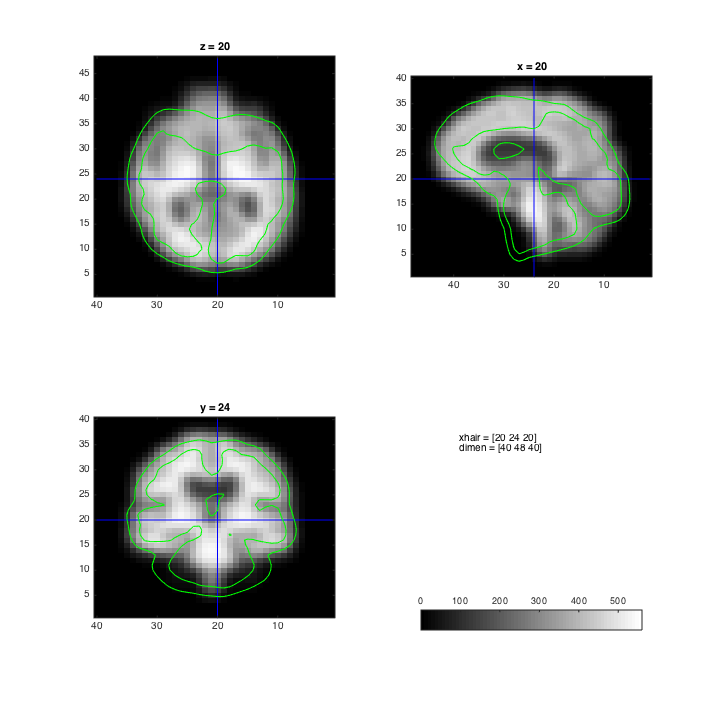
\includegraphics[width=.8\linewidth]{../img/314_a}}{\caption[p3.1.4 Before Registration]{Before Registration} \label{fig:314_a}}
				\ffigbox{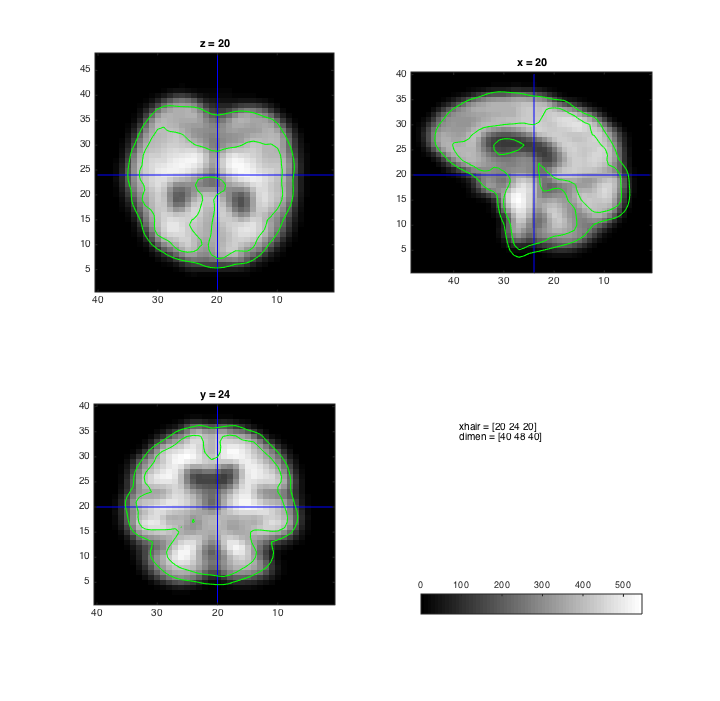
\includegraphics[width=.8\linewidth]{../img/314_b}}{\caption[p3.1.4 After Registration]{After Registration}\label{fig:314_b}}
			\end{floatrow}
		\end{figure}
		
		%		\lstinputlisting{../p314.m}
		
		
		\subsection*{3.1.5  Multi-Resolution Affine Registration}
		Using the script \lstinline|'p315.m'|, demonstrate another method for registration that to compute the transformation between two images, \lstinline|'sub001_mri.nii'| and \lstinline|'sub003_mri.nii'|. This method down samples the images for fast registration between them and gradually increases the resolution of the images, using the coordinate transform just solved for as initial conditions for the next layer of registration. \\
		
		\begin{center}
			$ A = \left| \begin{array}{ccc}
				0.9674 &   0.1352   & 0.0159\\
				-0.1554 &   0.8860  &  0.3120\\
				0.0171 &  -0.2672  &  1.0999 \end{array} \right| $
			$ b = \left| \begin{array}{c}
				-5.5977 \\
				-2.8699 \\
				7.9202 \end{array} \right| $		
		\end{center}
		
		\begin{figure}[!h]
			\begin{floatrow}
				\ffigbox{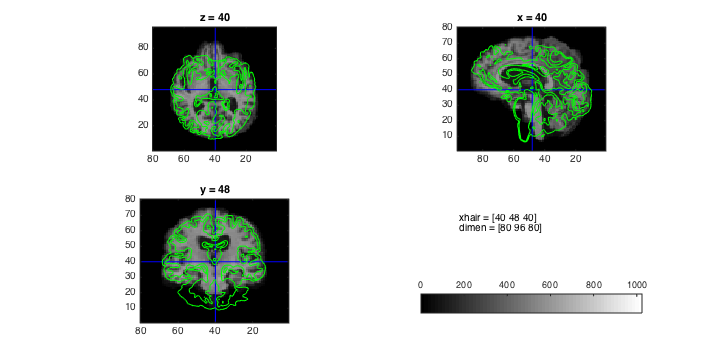
\includegraphics[width=.8\linewidth]{../img/315_a}}{\caption[p3.1.5 Before Multi-Layered Registration]{Before Multi-Layered Registration} \label{fig:315_a}}
				\ffigbox{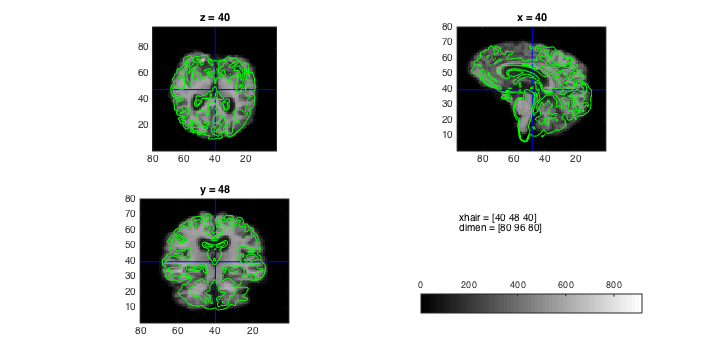
\includegraphics[width=.8\linewidth]{../img/315_b}}{\caption[p3.1.5 After Multi-Layered Registration]{After Multi-Layered Registration}\label{fig:315_b}}
			\end{floatrow}
		\end{figure}
		
		%		\lstinputlisting{../p315.m}
		

		\subsection*{3.1.6 Speedups in the Objective Function}
		Using \lstinline|my_interp3_precompute| and \lstinline|my_interp3| for interpolation did nor result in a significant speedup. Using the \lstinline|tic; toc;| function in Matlab for \lstinline|myAffineRegMultiRes3D| with \lstinline|iter = [20 10 5]| and \lstinline|sigma = 1| for images \lstinline|'sub001_mri.nii'| and \lstinline|'sub002_mri.nii'|, we got a baseline time of $102.61$ seconds. By precomputing the gradient we got the time down to $95.03$ seconds. Replacing \lstinline|interpn| with \lstinline|my_interp3| however, increased the time to $173.45$ seconds.


		\subsection*{3.1.7 Baseline Groupwise Registration}
		Using \lstinline|iter = [20 10 5]; sigma = 1.; fixed_img = sub021-sub040;| \\
		We get \lstinline|min(meanov) = .2827; max(meanov) = 0.3110; Mean(meanov) = 0.3025;|. 
	


		\section*{3.2 Extensions to the Base Component}		
		
		\subsection*{3.2.1 Baseline Groupwise Registration}
		In this, histogram of moving and fixed was matched before finding optimum values of A and b. This method works the best if the intensity ranges of the images are different. So to test it, we used sub0021 as our fixed image, and used sub001, sub002 and sub003 as moving images. Before matching, mean overlap was \lstinline|0.2399| and after matching, it improved to \lstinline|0.2624|. However, when this scheme was applied to all the images, no improvement was seen. This is because histogram matching leads may lead to loss in intensity information. So method of histogram matching is unpredictable.\\
		Source code: \lstinline|myHistMatch.m|
		
		\subsection*{3.2.2 Registration to an Unbiased Population-Derived Template}
		At 5 iterations, provided an improvement to mean overlap results relative to images with poor registration results (\lstinline|min(meanovl) = 0.2827|), but did not improve results for images with good registration results (\lstinline|max(meanovl) = 0.3110|). Multi-resolution affine transformation seems to be good enough that an average template doesn't offer much improvement.\\
		Source code:  \lstinline|p322.m|		
		
		\subsection*{3.2.3 Defining a Mask}
		Using the given segmentations for training images, mask template was derived by using the unbiased population approach (\lstinline|p323mask.m|). This mask was used to compute objective function. $J(Ax+b)$ was computed only at those points where $mask \neq 0$. This increased the computation speed significantly and allowed optimization of objective function at the highest resolution. This gave significant improvement in mean overlap of the images increasing it to $0.3643$ from $0.3111$ with sub030 used as the fixed image.\\
		When generating the mask template, we notice that the mean overlap goes down and then it becomes a constant. Initial template generated by just averaging the segmentation gives 0.3643 of mean overlap which goes down to 0.3468 after using the template generated after second iteration, and then it becomes constant for the templates generated in later iterations. $A0 = 0.3643$, $A1 = 0.3513$, $A2 = 0.3468$, $A3 = 0.3468$, $A4 = 0.3468$, $A5 = 0.3468$.\\
		Source code: \lstinline|myAffineObjective3DwithMask.m| and \lstinline|myAffineMultiRes3DwithMask.m| and \lstinline|p323mask.m|
		
		
		\subsection*{3.2.4 Analytic Hessian Computation}
		The analytic hessian was computed within the objective function. For sub001 as the fixed image and sub002 as the moving image, maximum relative error was found to be $0.0584\%$. This shows that the results are still valid.  This enhancement resulted in a significant speedup compared to \lstinline|myAffineObjective3D.m|. This increased the speed of registration dramatically allowing us to run additional iterations at higher resolutions. Before the enhancement, we saw a baseline registration take $95.03 seconds$. After the enhancement, we saw the time drop to $33.81 seconds$. This speedup also enabled us to run many more tests as can be seen below
		Source code:  \lstinline|myAffineObjective3DwithHessian.m|,  \lstinline|p324.m| \\\\
		
		
		\section{Table of results for enhancements}
		\begin{tabular}{|p{5cm}|p{8cm}|p{2cm}|}
			\hline
			Name & Description& meanovl \\ \hline \hline
			3.2.1 Histogram Matching & Match histogram of fixed and moving image before performing registration & 0.2846 \\ \hline
			3.2.2 Registration to an Unbiased Population-Derived Template & Create template by averaging input image intensities and registering to this average iteratively (j=5) & A0=0.2896 A5=0.3014\\ \hline
			3.2.3 Defining a Mask & Set intensity to 0 for regions outside of the hippocampus using the segmentation images & .3643 \\ \hline
			3.2.4 Analytic Hessian Computation & Compute analytic Hessian in the objective function to speed up computations and perform more iterations at higher resolution & 0.3111 \\ \hline
		\end{tabular}

		
		\section{Experiments}
		
		\begin{tabular}{ | p{1.8cm} | p{1.5cm} | p{1.5cm} | p{1.5cm} | p{1.7cm} | p{1.5cm} | p{1.7cm} | p{1.5cm} |  }
			\hline 
			Fixed & Iter & Sigma & Hessian & Histogram & Mask & Template & Overlap \\ \hline \hline 
			sub021 & [20,10,0] & 1 & Yes & Yes & No & No & 0.2306 \\ \hline
			sub030 & [20,10,0] & 1 & Yes & Yes & No & No & 0.2529 \\ \hline
			sub030 & [20,10,0] & 1 & No & No & No & No & 0.2889 \\ \hline
			sub021 & [20,10,5] & 1 & Yes & No & No & No & 0.3067 \\ \hline
			sub030 & [20,10,5] & 1 & No & No & No & No & 0.3106 \\ \hline
			sub030 & [20,10,5] & 1 & Yes & No & No & No & 0.3110 \\ \hline
			sub021 & [20,10,5] & 2 & No & No & No & No & 0.2798 \\ \hline
			sub030 & [20,10,5] & 2 & No & No & No & No & 0.2875 \\ \hline
			sub030 & [40,20,5] & 1 & Yes & No & No & No & 0.3105 \\ \hline
			sub030 & [40,20,5] & 2 & Yes & No & No & No & 0.2921 \\ \hline
			sub030 & [80,40,5] & 1 & Yes & No & No & No & 0.3111 \\ \hline
			sub030 & [80,40,5] & 1 & Yes & Yes & No & No & 0.2846 \\ \hline
			sub030 & [80,40,5] & 2 & Yes & No & No & No & 0.2909 \\ \hline
			sub030 & [80,40,5] & 2 & Yes & Yes & No & No & 0.2536 \\ \hline
			sub030 & [80,40,20,5] & 1 & Yes & No & No & No & 0.3107 \\ \hline
			\textbf{sub030} & \textbf{50} & \textbf{1} & \textbf{Yes} & \textbf{No} & \textbf{Yes} & \textbf{No} & \textbf{0.3643} \\ \hline
			sub030 & 50 & 1 & Yes & Yes & Yes & No & 0.3643 \\ \hline
			A5\_template & [20, 10, 5] & 1 & Yes & No & No & Yes & 0.3014 \\ \hline
		\end{tabular}
		




	\end{par}
	

\end{document}
    
